
\section{Reducing demo data}
\label{sec:reducing_demo_data}
In this section we show how to reduce the demo datasets within the
distribution kit of the molecfit pipeline. The procedure can be
extended to any valid dataset.

{\bf Important note. The EDPS workflow associated with pipeline
version \pipelinevers\ supports reduced 1 dimensional spectra in IDP
format \footnote{Binary table that follows the ESO science archive
standards. They can be recognized by the header keyword {\tt PRODCATG=SCIENCE.SPECTRUM}. Examples can be obtained by downloading a
science product from the ESO science archive at:\\
\url{https://archive.eso.org/scienceportal/home}} of the following
instruments: XSHOOTER, UVES, ESPRESSO, GIRAFFE, FORS. Additionally,
VISIR data with product category {\tt SPC\_OBS\_LMR\_TAB} as shown in
the header keyword {\tt HIERARCH ESO PRO CATG}. Also, spectra must
have minimum wavelenght greater than 650 nm, as indicated in the
header keyword {\tt WAVELMIN}.}



Follow this procedure to quickly reduce \instname\ demo data. We
assume that the \edps, \edpsgui, the \instname\ pipeline and its
associated demo data are installed in your system. For general
instructions on how to install \edps\ and the pipeline, see Section
{\ref{sec:installation} or please visit:\\
\href{https://www.eso.org/sci/software/pipe_aem_main.html}{https://www.eso.org/sci/software/pipe\_aem\_main.html}.

\subsection{Setting the workflow}
Proceed as follows:
\begin{enumerate}

\item If not done already, activate the \edps\ virtual environment, defined during installation (Sect. \ref{sec:installation}).
\item Start the \edpsgui\ dashboard by typing:
\begin{verbatim}
 edps-gui
\end{verbatim}

The \edpsgui\ dashboard will start in a browser window (Figure \ref{fig:dashboard}). 


\begin{figure}[h!]
\centering
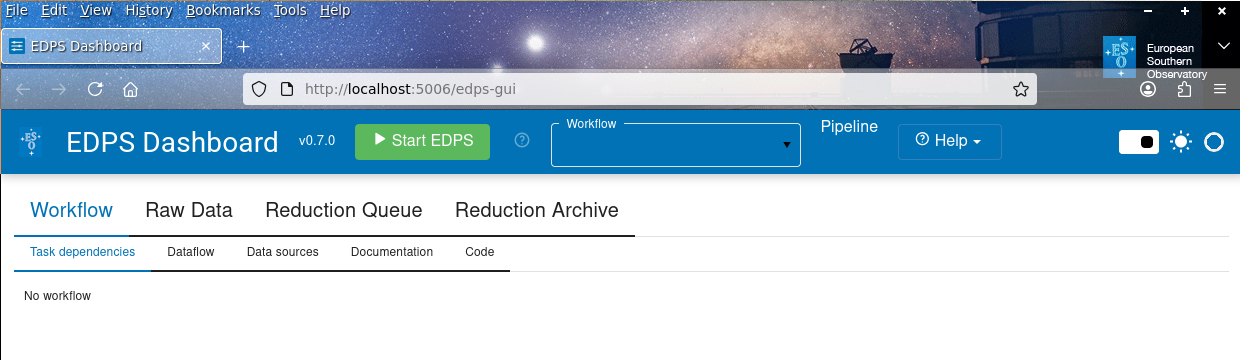
\includegraphics[width=0.9\textwidth]{../common/figures/dashboard.jpg}
\caption{The empty \edpsgui\ Dashboard; the underlying \edps\ engine has not yet been started and no workflow has been loaded.}
\label{fig:dashboard}
\end{figure}

\item Optionally, before starting \edps, one can specify new settings by pressing Help --> Settings (Figure \ref{fig:help_settings}).

\begin{figure}[h!]
\centering
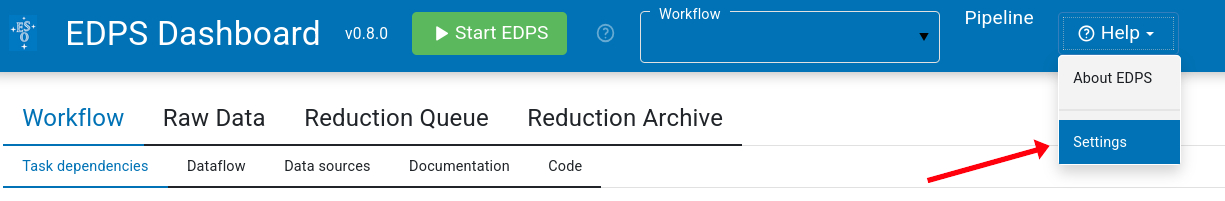
\includegraphics[width=0.9\textwidth]{../common/figures/help_settings.jpg}
\caption{The ``Help'' --> ``Settings'' menu.}
\label{fig:help_settings}
\end{figure}

\item On the browser window with the dashboard, press the button `Start EDPS`.

\begin{figure}[h!]
\centering
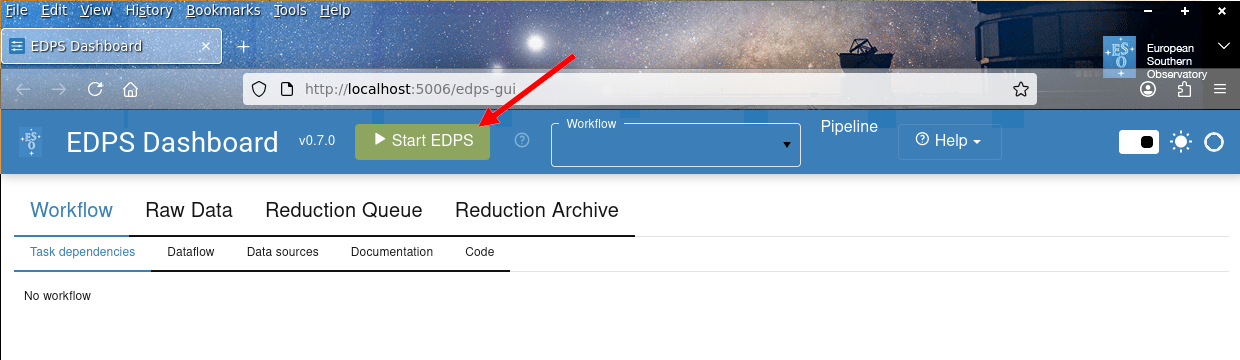
\includegraphics[width=0.9\textwidth]{../common/figures/start_edps.jpg}
\caption{The ``Start EDPS'' button.}
\label{fig:start_edps}
\end{figure}


\item Choose the \wkfname\ workflow from the list in the 'Workflow' field. The workflows offered in this selector depend on
the installed pipelines.
The graphic workflow representation will appear as in Figure \ref{fig:select_workflow}.



\begin{figure}[h!]
\centering
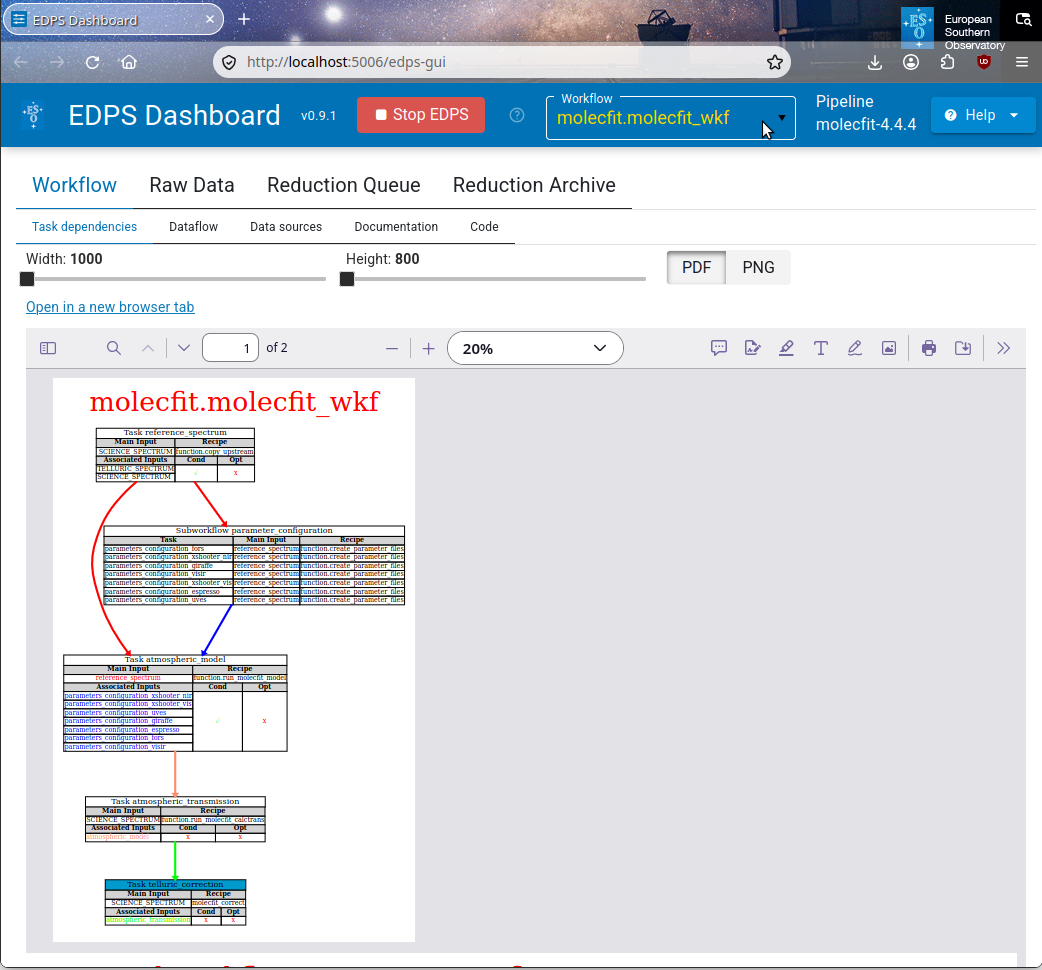
\includegraphics[width=0.9\textwidth]{../instrument_tutorial/figures/select_workflow.jpg}
\caption{The \edpsgui\ with the \instname\ workflow loaded.	}
\label{fig:select_workflow}
\end{figure}

\end{enumerate}

\subsection{Selecting the input data}

\begin{enumerate}
\item Press `Raw Data` to enter the corresponding tab, as in Figure \ref{fig:raw_data}.


\begin{figure}[h!]
\centering
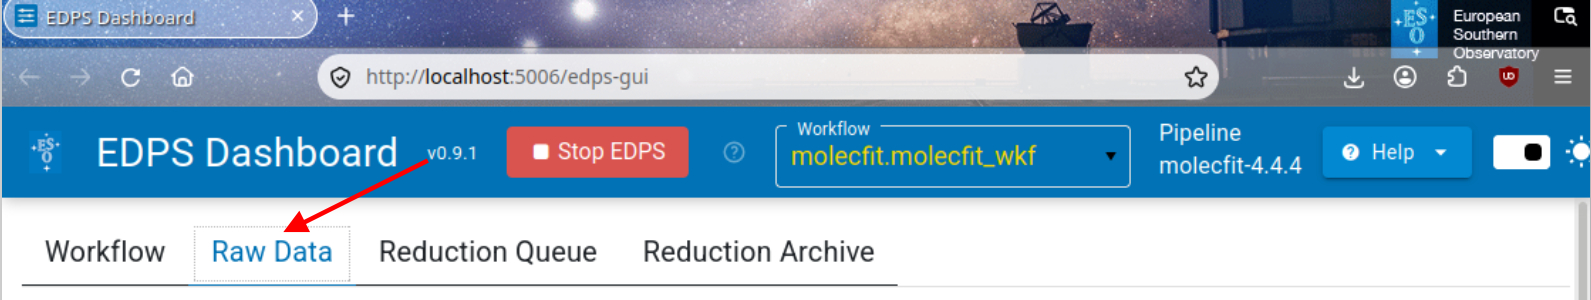
\includegraphics[width=0.9\textwidth]{../instrument_tutorial/figures/raw_data.jpg}
\caption{How to select RAW data Tab.}
\label{fig:raw_data}
\end{figure}
 	
\item Press `Select Inputs`. A selection window will appear that allows to select data that are stored on a local disk (Figure \ref{fig:select_input}).


\begin{figure}[h!]
\centering
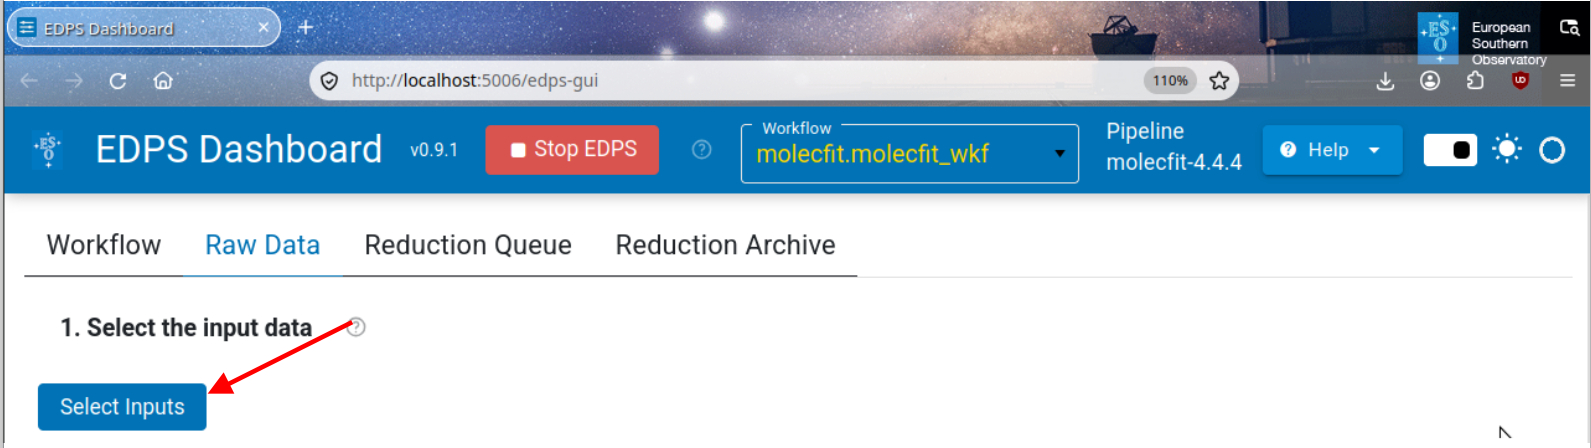
\includegraphics[width=0.9\textwidth]{../instrument_tutorial/figures/select_input.jpg}
\caption{How to select input data.}
\label{fig:select_input}
\end{figure}
 
\item (Optional). Select the reduction target, configure the workflow parameter and specify the association preferences. 
These steps are optional. For more information see Section \ref{sec:configuration_overview}.


\item Press `Create Datasets`. A list of datasets appears, one line for each set of science data (Figure \ref{fig:create_datasets}).
	
   

\begin{figure}[h!]
\centering
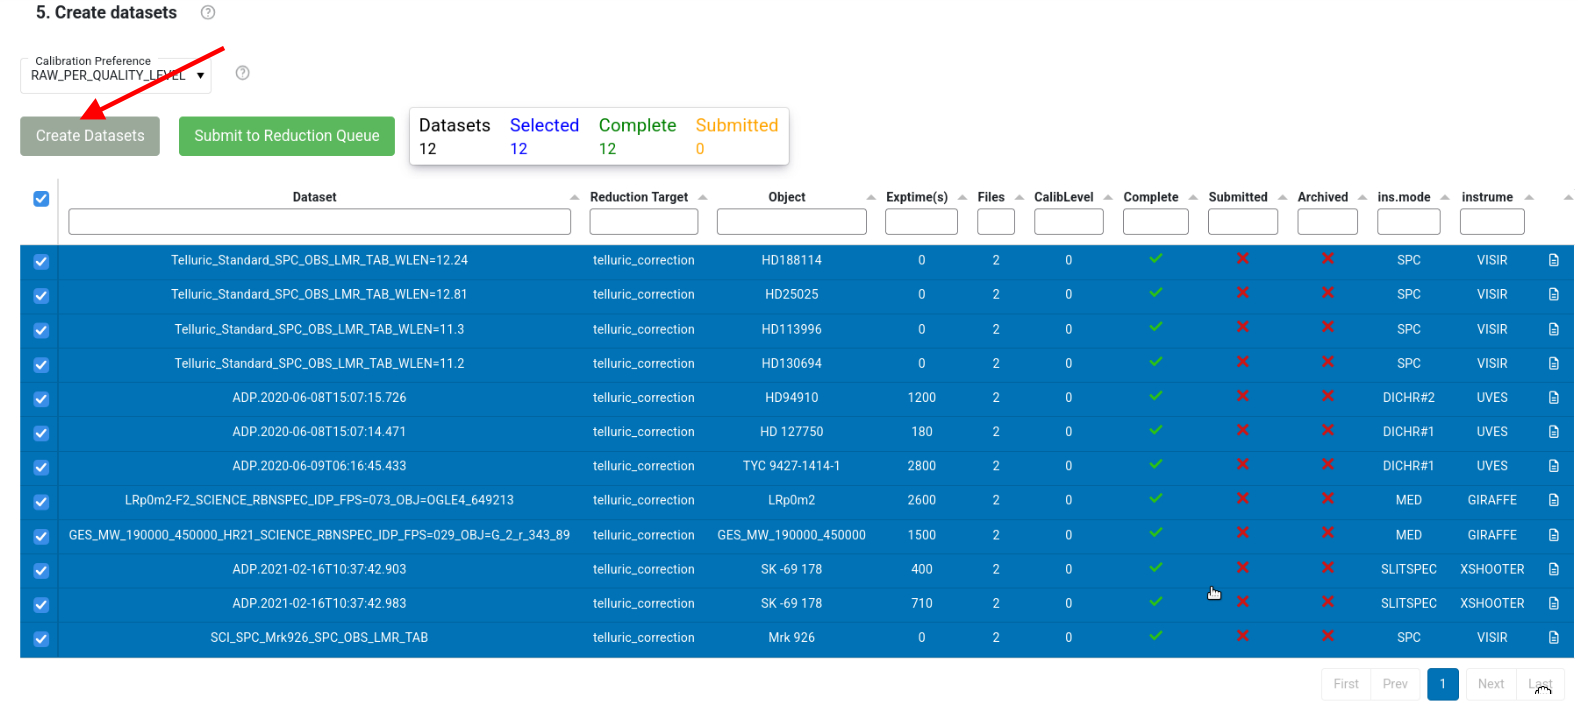
\includegraphics[width=0.9\textwidth]{../instrument_tutorial/figures/create_datasets.jpg}
\caption{How to inspect the input data directory to create datasets.}
\label{fig:create_datasets}
\end{figure}
\item Choose the datasets that should be processed (Figure \ref{fig:send})
	
\begin{figure}[h!]
\centering
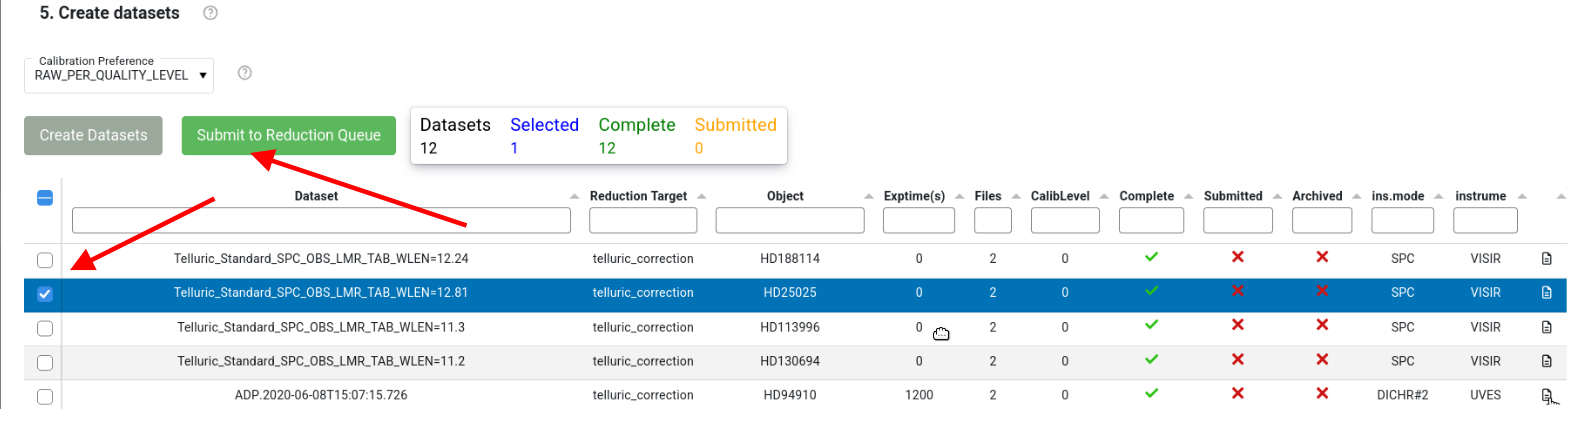
\includegraphics[width=0.9\textwidth]{../instrument_tutorial/figures/send.jpg}
\caption{How to send the selected datasets to the Reduction Queue for processing.}
\label{fig:send}
\end{figure}
and send them to the data reduction queue by pressing `Submit to Reduction Queue`. Note that this action does not start the 
reduction automatically.

\end{enumerate}

\subsection{Start the reduction}

\begin{enumerate}

\item Press the `Reduction Queue` tab (Figure \ref{fig:reduction_queue}).


\begin{figure}[h!]
\centering
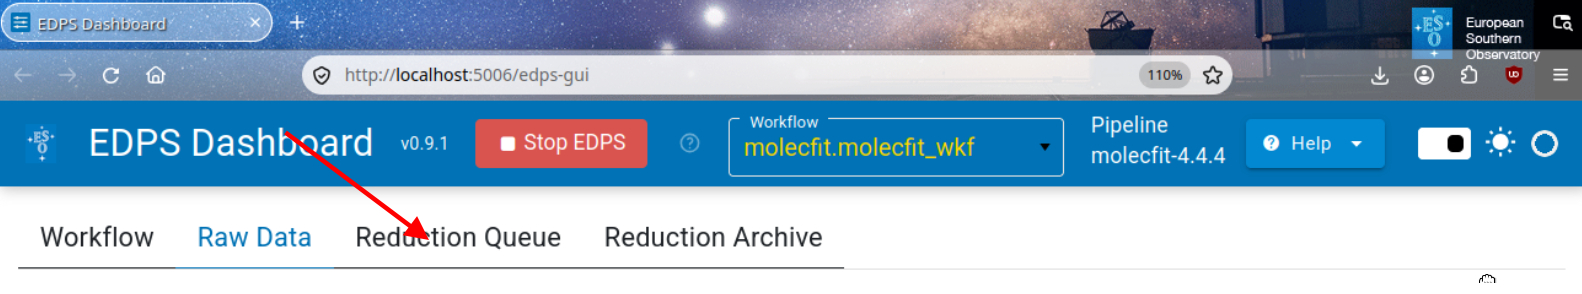
\includegraphics[width=0.9\textwidth]{../instrument_tutorial/figures/processing_queue.jpg}
\caption{How to select Reduction Queue tab.}
\label{fig:reduction_queue}
\end{figure}

\item Select the datasets you'd like to reduce.

\item (Optional). Configure the workflow and recipe parameters by pressing the wheel 
button 
\includegraphics[width=0.8cm]{../common/figures/configure_dataset.jpg}
to open the configuration editor. See
Section \ref{sec:configuration_editor} for more information on the
configuration editor.
 
\item Press the `Reduce` button (Figure \ref{fig:reduce}). The selected data will now be processed with the configured parameters.


\begin{figure}[h!]
\centering
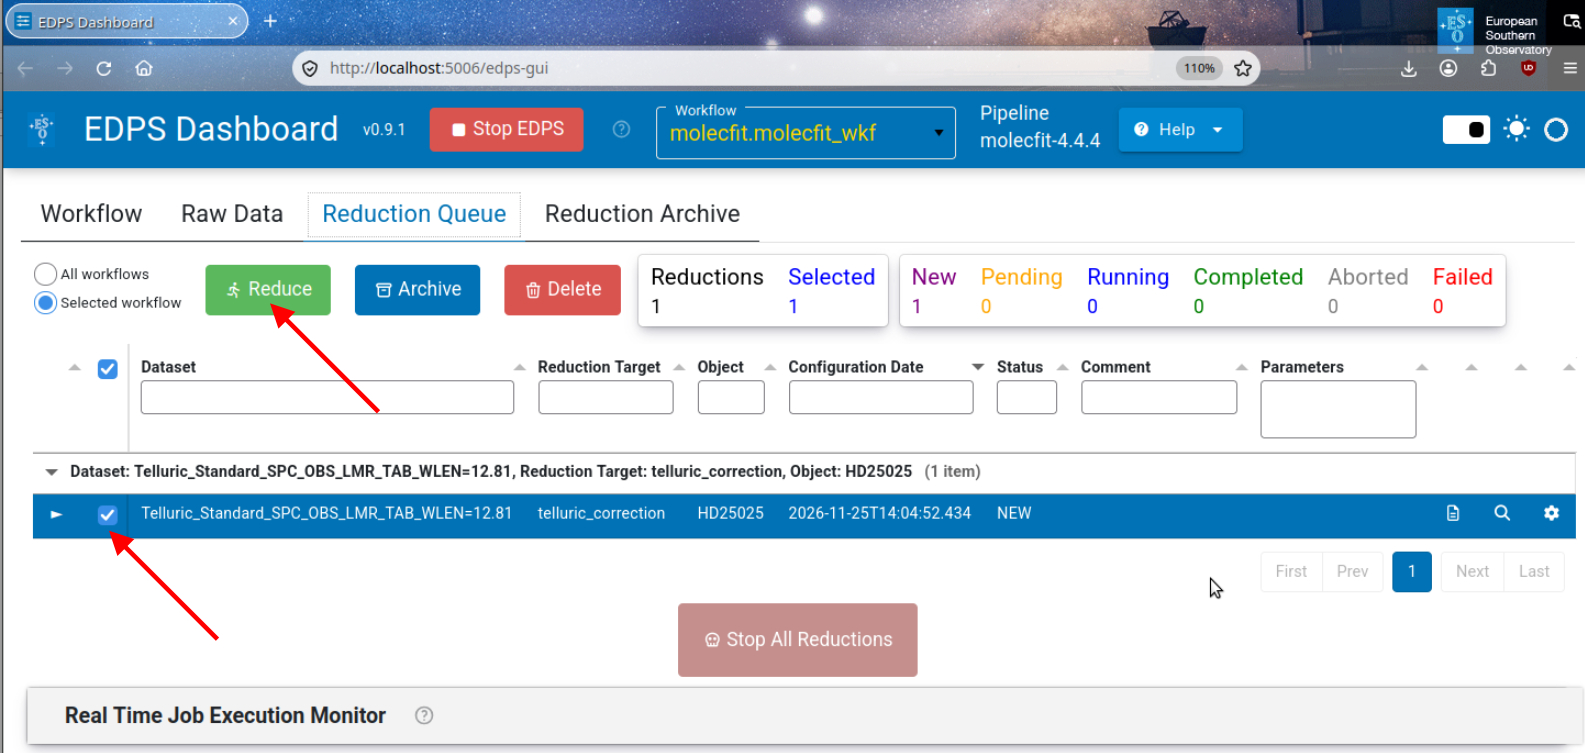
\includegraphics[width=0.9\textwidth]{../instrument_tutorial/figures/reduce.jpg}
\caption{Reduce.}
\label{fig:reduce}
\end{figure}


\end{enumerate}

Congratulations! You reduced your first data with the \edps\
dashboard! All the reduced data are saved in the EDPS\_data directory
specified when executing \edpsgui\ for the first time.


 
\subsubsection{Quality plots}
It is possible to inspect the information on each job, such as quality plots showing the products (for the most important jobs and products), the list of inputs and output files, the recipe parameters and logs. 
All the information on the job processing can be inspected from the `Reduction Queue` window. While quality plots are produced only for completed jobs, the other relevant information is available also for failed jobs.

The information associated for the main product can be inspected by pressing the magnifying glass symbol at the right side of each dataset.
To inspect the information associated to other individual jobs (e.g., calibrations), proceed as follows: 

\begin{itemize}
 \item Expand the desired dataset by pressing the black arrow on its left. The list of jobs will appear with the associated status (COMPLETED, RUNNING, PENDING, MISSING, ABORTED, FAILED)
 \item Press the  magnifying glass symbol at the right side of the job you want to inspect. 
\end{itemize}

 
\begin{figure}[h!]
\centering
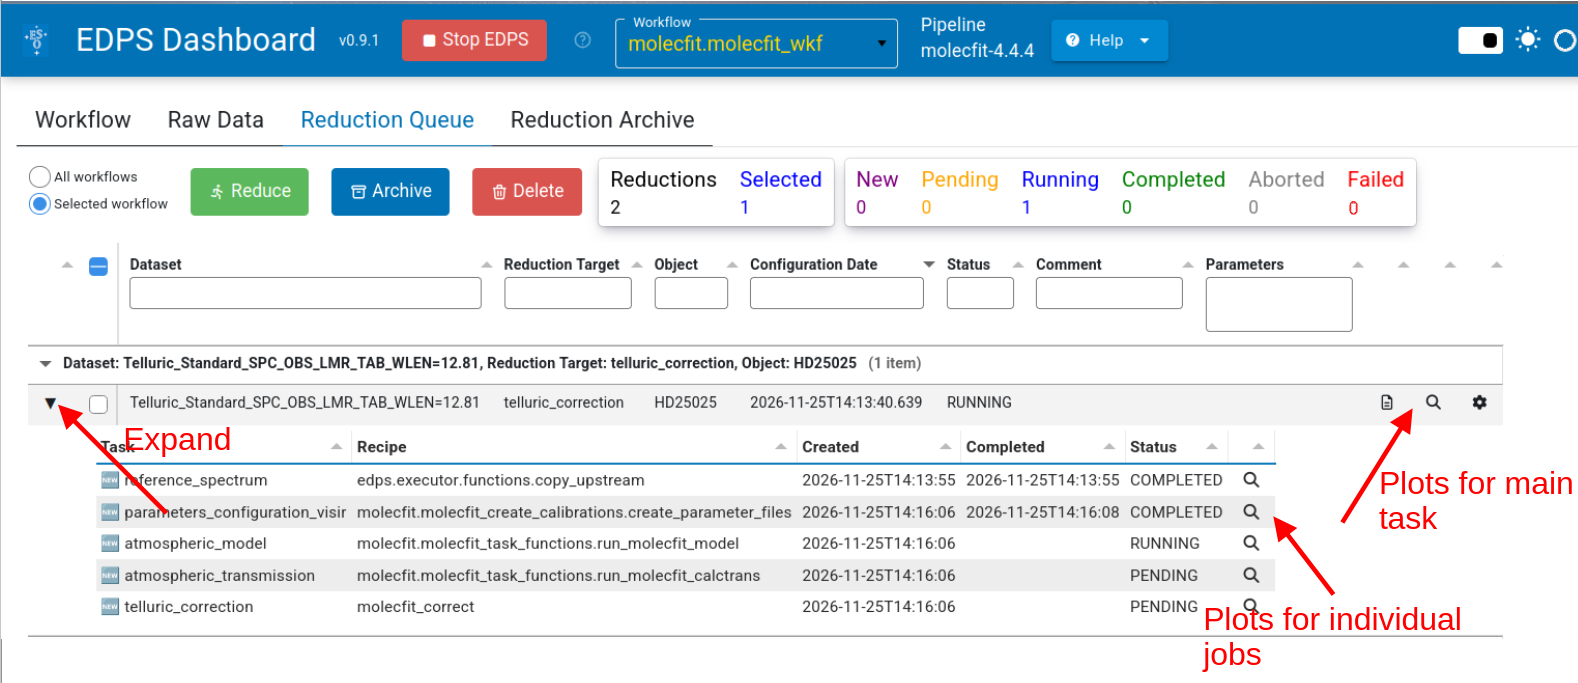
\includegraphics[width=0.9\textwidth]{../instrument_tutorial/figures/show_reports.jpg}
\caption{How to look for job information from the Reduction Queue tab.}
\label{fig:show_reports}
\end{figure}


\subsection{Exporting the final products}
\label{sec:export_final_products}



Completed reductions can be 'Archived' (i.e. declared 'completed'
because no more work is needed) and removed from the Reduction
Queue. Additionally, even if all products for all tasks are saved in
the EDPS\_data directory, the most important products can be
`exported' to a desired location.

To do so, proceed as follows:

\begin{enumerate}
\item In the `Reduction Queue` tab, select the dataset and the dataset
  for which you want to export the final products, and press the
  'Archive' button.
  
\begin{figure}[h!]
\centering
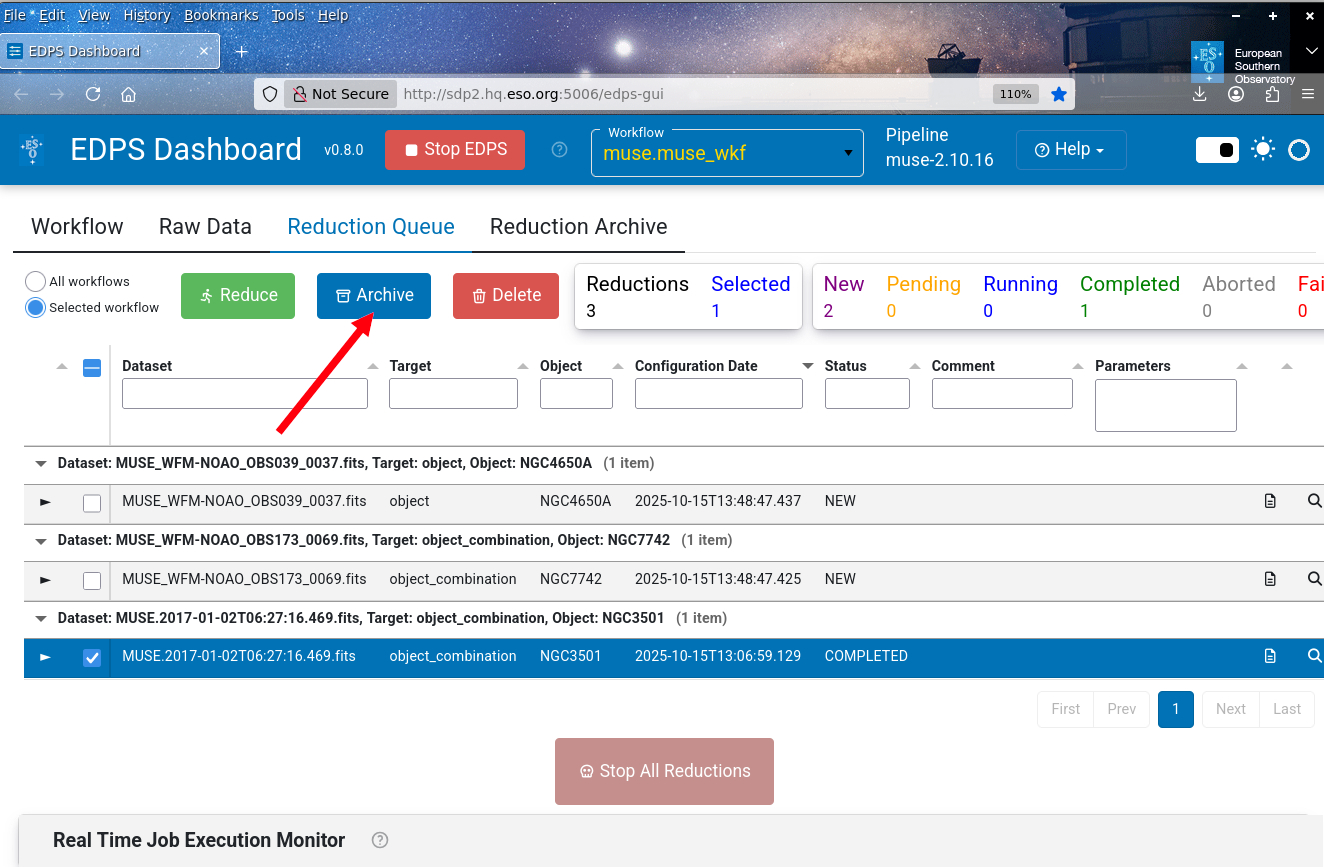
\includegraphics[width=0.8\textwidth]{../instrument_tutorial/figures/archive.jpg}
\caption{How to archive a completed reduction from the Reduction Queue tab.}
\end{figure}



\item Go in the Reduction Archive tab and click on the 'Export'
  button. A new tab window appears where you can indicate the directory
  you want to copy your final products; finally press "Export" to copy
  the data.


\begin{figure}[h!]
\centering
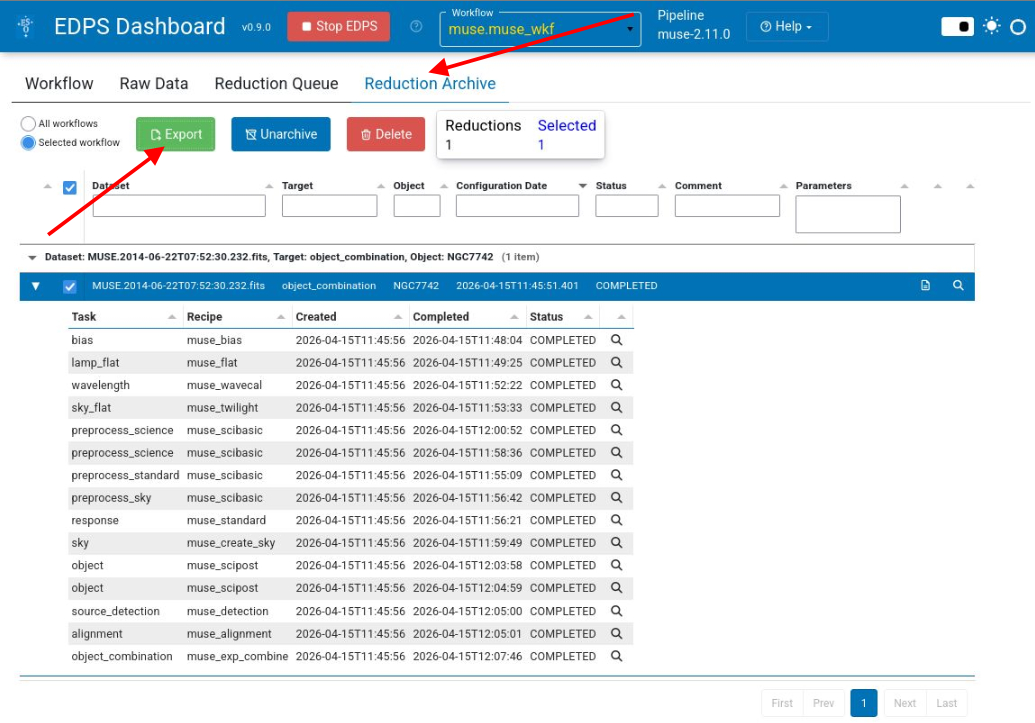
\includegraphics[width=0.8\textwidth]{../instrument_tutorial/figures/export1.jpg}
\caption{The reduction archive tab. This table contains all the different configurations of datasets that are declared "finished" and removed from the Reduction Queue. From this page, the user can export the most important files into a desired local directory.}
\end{figure}



\begin{figure}[h!]
\centering
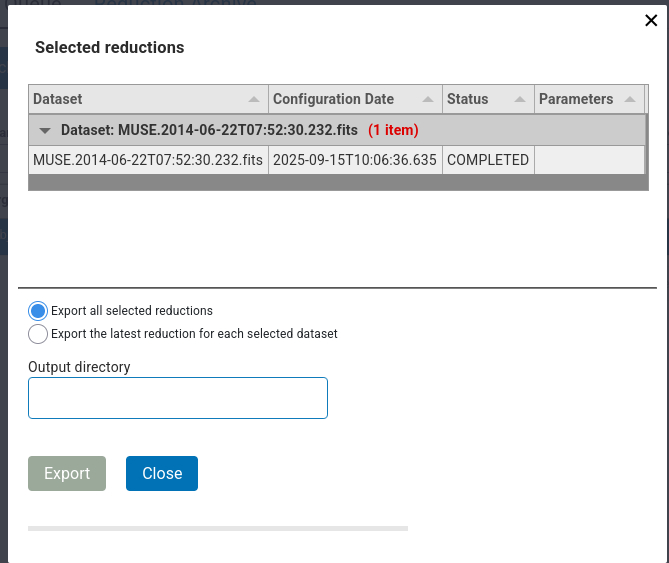
\includegraphics[width=0.7\textwidth]{../instrument_tutorial/figures/export2.jpg}
\caption{The EXPORT dialogue window, where the user can decide which reduced configuration to save and where.}
\end{figure}

\end{enumerate}

 
 
Exported products are organized by `DATASET` (named as the first
scientific exposure of the dataset), and `TIMESTAMP` (time of start of
reduction)

The final products saved in the specified directory are: 



{\bf DESCRIBE HERE THE LIST OF THE FINAL EXPORTED PRODUCTS}
\begin{itemize}
\item product 1 ...
\item product 2 ...
\end{itemize}
